\chapter{Cơ sở lý thuyết} \label{chap:theory}
    \section{High-Level Synthesis - HLS}
    Công cụ Xilinx Vivado HLS chuyển đổi từ đặc tả C sang hiện thực ở mức độ biến đổi thanh ghi (RTL implement). Từ đó có thể tổng hợp thành một Xilinx FPGA. 
        \subsection{Lợi ích của HLS}
        \textbf{HLS là cầu nối giữa phần cứng và phần mềm với những lợi ích hàng đầu sau:}
        \begin{itemize}
            \item Cải thiện năng suất cho những người thiết kế phần cứng.
            Những người thiết kế phần cứng có thể làm việc ở mức độ trừu tượng cao hơn trong khi vẫn tạo được phần cứng có hiệu năng cao.
            \item Cải thiện hiệu năng hệ thống đối với những người thiết kế phần mềm.
            Người phát triển phần mềm có thể gia tốc những phần nặng về tính toán trog giải thuật của họ trên một mục tiêu mới, FPGA.
        \end{itemize}
        \textbf{Việc sử dụng phương pháp thiết kế HLS cho phép:}
        \begin{itemize}
            \item Phát triển giải thuật bằng ngôn ngữ C.
            \item Kiểm chứng ở mức ngôn ngữ C.
            Xác thực tính đúng đắn của hàm trong thiết kế nhanh hơn so với ngôn ngữ đặc tả phần cứng truyền thống.
        \end{itemize}
        \subsection{Vivado HLS}
        Công cụ Xilinx Vivado HLS tổng hợp một hàm C thành một khối IP mà có thể tích hợp với hệ thống phần cứng. Nó liên kết chặt chẽ với những công cụ thiết kế còn lại của Xilinx để tạo ra hiện thực tối ưu cho giải thuật C.
        
        Thiết kế Vivado HLS bao gồm các bước sau (hình \ref{fig:vivadohlsflow}):
        
        \begin{figure}[htp]
    		\centering
     		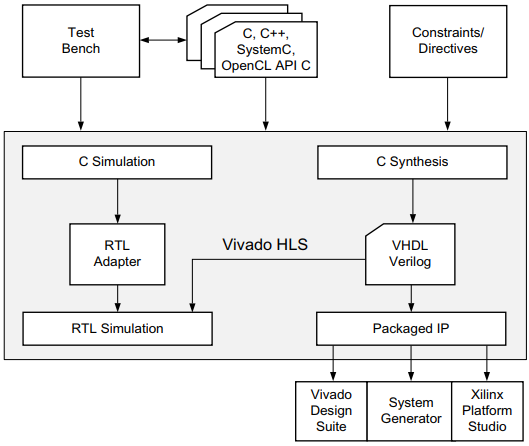
\includegraphics[scale=.8]{images/vivadohlsflow.png}
    		\caption{Sơ đồ sử hoạt động Vivado HLS}
    		\label{fig:vivadohlsflow}
    	\end{figure}
    	
        \begin{enumerate}
            \item Biên dịch, thực thi (mô phỏng) và debug giải thuật C.
            Trong HLS, chạy một chương trình đã được biên dịch tức là chạy mô phỏng C. Thực thi một hàm được mô phỏng bằng C để chắc chắn rằng giải thuật đó làm đúng chức năng.
            \item Tổng hợp giải thuật C thành hiện thực RTL.
            \item Sinh những báo cáo toàn diện và phân tích thiết kế.
            \item Kiểm chứng và đóng gói hiện thực RTL thành khối IP.
        \end{enumerate}
        \subsection{Sử dụng Vivado HLS}
    \section{Vivado IDE}
    \section{Bo mạch Ultra96}
    \section{PYNQ Framework}
        \subsection{Pynq là gì?}
        PYNQ, Python Productivity for Zynq, là một dự án mã nguồn mở của Xilinx giúp dễ dàng thiết kế những hệ thống nhúng với Xilinx Zynq\cite{zynq} Systems on Chips (SoCs).
		Bằng việc sử dụng ngôn ngữ Python và các thư viện, người thiết kế có thể khai thác những thế mạnh của FPGA (hay programmable logic) cũng như của bộ vi xử lí trên Zynq xây dựng những hệ thống nhúng thú vị và hiệu quả. Đặc biệt, Pynq cho phép những kiến trúc sư, những kỹ sư và những người lập trình về hệ thống nhúng có thể sử dụng thiết bị Zynq mà không phải sử dụng đến các công cụ thiết kế ASIC-style.

		\begin{figure}[htp]
    		\centering
     		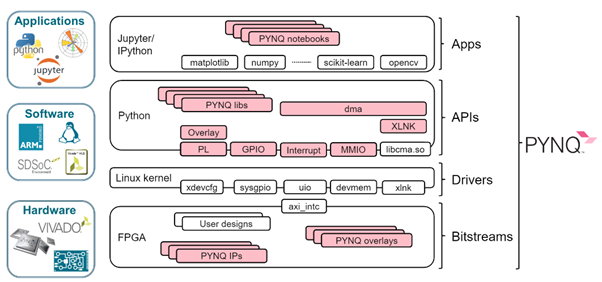
\includegraphics[scale=.7]{images/pynq.png}
    		\caption{Sơ đồ khối của Pynq}
    		\label{fig:pynqblockdiagram}
    	\end{figure}

		Pynq đạt được điều đó bởi:
		\begin{enumerate}
			\item Những mạch lô-gíc lập trình được xem như những thư viện phần cứng hay còn gọi là overlays. Những overlays này tương tự như những thư viện phần mềm. Một kỹ sư phần mềm có thể lựa chọn những overlay phù hợp nhất với ứng dụng của mình. Một overlay có thể được truy cập thông của giao diện ứng dụng lập trình (API). Việc tạo một overlay mới đòi hỏi người kỹ sư có kiến thức về thiết kế mạch lô-gíc lập trình.
			\item Pynq sử dụng Python cho việc lập trình trên cả những vi xử lý và những overlay. Mà Python là một ngôn ngữ bậc cao rất hiệu quả. Ngày nay, C hay C++ là nhũng ngôn ngữ lập trình cho hệ thống nhúng phổ biến nhất. Nhưng, Python là ngôn ngữ có mức độ trừu tượng tốt hơn và mang lại hiệu suất cao hơn cho người lập trình. Tuy nhiên không có sự lựa chọn nào là tốt tuyệt đối. Pynq sử dụng CPython - được viết bằng C, và tích hợp với hàng ngàn thư viện C. Nếu hướng tới tăng hiệu suất lập trình thì nên sử dụng môi trường Python và nếu muốn tăng hiệu năng thì lập trình C nên được ưu tiên.
			\item Pynq là dự án mã nguồn mở hướng tới có thể hoạt động 	trên bất kỳ nền tảng hay hệ điều hành nào. Đạt được điều này bằng việc thông qua kiến trúc trên nền web, còn được gọi là browser agnostic. Nó tích hợp nền tảng mã nguồn mở Jupyter notebook để chạy một nhân Interactive Python (IPython) và một web server trực tiếp trên vi xử lý ARM của thiết bị Zynq.
		\end{enumerate}
        
        \subsection{PYNQ Overlays}\label{subsec:overlayintro}

        Thiết bị Zynq là một hệ thống trên chíp gồm hai phần cơ bản là bộ vi xử lý (gọi là Processing System hay PS) và tích hợp với phần FPGA (còn gọi là Programmable Logic hay PL). Phần PS bao gồm hàng tá những thiết bị ngoại vi (memory controllers, USB, Uart, IIC, SPI,...) và có thể mở rộng ra những IP phần cứng bổ sung trên một overlay PL (xem hình \ref{fig:zynqblockdiagram}).

        \begin{figure}[htp]
    		\centering
     		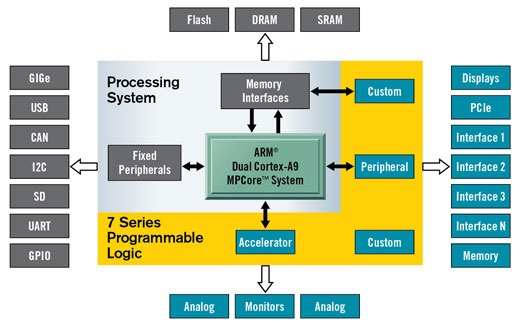
\includegraphics[scale=1]{images/zynq_block_diagram.jpg}
    		\caption{Sơ đồ khối của Zynq}
    		\label{fig:zynqblockdiagram}
    	\end{figure}

		Overlay, hay còn gọi là thư viện phần cứng, là những thiết kế FPGA. Nó mở rộng và kết nối phần PS của Zynq với phần PL. Overlay có thể được sử dụng để gia tốc một ứng dụng phần mềm hay tùy chỉnh nền tàng phần cứng cho phù hợp với những ứng dụng đặc thù.

		Ví dụ, xử lý ảnh là một ứng dụng điền hình, nơi mà FPGA có thể được sử dụng để gia tốc. Một người lập trình phần mềm có thể sử dụng một overlay tương tự như sử dụng thư viện phần mềm đề chạy một số hàm sử lý ảnh trên nền tảng FPGA. Những overlay có thể được tải lên FPGA một cách linh hoạt khi được yêu cầu, giống như một thư viện phần mềm. Những hàm xử lý ảnh riêng biệt có thể được hiện thực bằng những overlay khác nhau và được tải lên dựa vào yêu cầu từ Python.

		Pynq cung cấp một giao diện Python cho phép Python chạy trên phần PS có thể điều khiển những overlay chạy trên phần PL. Thiết kế FPGA là công việc đặc thù mà đòi hỏi sự hiểu biết của người kỹ sư về phần cứng. Những Pynq overlay có được tạo ra bời người thiết kế phần cứng và được gói lại với Pynq Python API. Người phát triển phần mềm có thể sử dụng giao diện Python đề lập trình và điều khiển những overlay phần cứng mà không cần tự tay thiết kế chúng. Điều này tương tự như sử dụng thư viện phần mềm được tạo ra bời những người phát triền nhiều kinh nghiệm.

		\subsection{Phương pháp thiết kế overlay}
		Đã được nêu lên trong phần \ref{subsec:overlayintro}, overlay tương tự như những thư viện phần mềm. Một người lập trình có thể tải overlay vào phần PL để cung cấp những chức năng mà ứng dụng cần.

		Một overlay là một lớp những thiết kế PL. Những thiết kế PL này luôn được tối ưu hóa cho một công việc nhất định. Tuy nhiên cũng có những overlay được thiết kế để có thể tùy chình và sử dụng lại cho những tập ứng dụng nhất định. Một Pynq overlay có giao diện Python. Điều này cho phép người lập trình có thể sử dụng nó như một gói Python.

		Người lập trình phần mềm có thể sử dụng overlay mà không tạo ra chúng vì điều này cần hiểu biết về thiết kế phần cứng. Tuy nhiên có một số công việc cần tới quá trình tạo một overlay:
		\begin{itemize}
			\item Tích hợp Python và C.
			\item Tạo API chó Python overlay.
			\item Thiết lập board
			\item Tạo gói Python
		\end{itemize}

		Phần này sẽ chỉ ra quá trình để tạo một overlay và tích hợp nó vào Pynq.

		\subsubsection{Thiết kế overlay} 
		Một overlay bao gồm hai thành phần; phần thiết kế PL (bitstream) và phần sơ đồ khối (tệp tcl). Thiết kế overlay là công việc đặc thù của kỹ sư phần cứng. Phần này đòi hỏi đến kiến thức về xây dựng thế thống Zynq cùng với các công cụ thiết kế Vivado.

		\textbf{Thiết kế PL}

		Phần mềm Xilinx Vivado được sử dụng cho việc tạo một thiết kế Zynq. Một bitstream hay một tệp nhị phân sẽ được sinh ra và được sử dụng cho lập trình trên Zynq PL.
		Những thiết kế phần cứng hỗ trợ lập trình trong những IP (Intellectual property), được sử dụng trong những Pynq overlay. Khi IP được tạo ra, thiết kế PL sẽ được thực hiện giống như bất kỳ thiết kế Zynq nào. IP trong overlay, được điều khiển bởi Pynq, sẽ được ánh xạ vùng nhớ và gắn với GPIO. Pynq cung cấp thư viện để tương tác với thiết kế PL và được sử dụng để tạo driver.

		\textbf{Tệp overlay Tcl}
		
		Tệp Tcl từ Vivado IP được sử dụng bởi Pynq để tự động xác định tùy chỉnh hệ thống Zynq. IP bao gồm phiên bản, ngắt, reset, và các tín hiệu khác. Dựa trên những thông tin này, một phần của việc tùy chỉnh hệ thống được tự động tinh chỉnh từ Pynq, những driver có thể tự động được gán, một số đặc điểm có thể được kích hoạt hay gỡ bỏ và những tín hiệu có thể được kết nối đến các phương thức trả lời của Python.

		Tệp Tcl phải được sinh ra và cung cấp cùng với tệp nhị phân (bitstream) như là một phần của overlay. Tệp Tcl có thể được sinh ra trong công cụ Vivado bằng cách xuất sơ đồ khối tích hợp IP ( IP Integrator block diagram) tại cuối quá trình thiết kế overlay. Tệp Tcl phải được cung cấp cùng với tệp nhị phân khi tải overlay. Lớp Pynq PL sẽ tự động phân tích tệp Tcl.

		Tên của tệp Tcl cần được giống với tên của tệp nhị phân. Ví dụ 	my\_overlay.bit và my\_overlay.tcl.
	
	\section{xfopecv}
	
	\section{Tổng quang về nhận dạng biển số xe}
		\subsection{Khái niệm về hệ thống nhận dạng biển số xe}
		Hệ thống nhận dạng biển số xe là hệ thống có khả năng phân tích hình ảnh và xác định vùng chứa biển số trên xe, thông qua video, thiết bị ghi hình và hình ảnh.
		\subsection{Lịch sử và phát triển}
		Năm 1992, công nghệ ALPR (Automatic License Plate Number) hay còn gọi là tự động nhận dạng biển số xe, được phát triển tại Đại học Cambridge ở Vương quốc Anh để ứng phó với chủ nghĩa khủng bố.
		
	    Đến năm 1996, công nghệ ALPR đã được hoàn thiện tại mỗi cổng phía tây Vương quốc Anh để đọc tất cả các biển đăng ký xe từ Ireland. Công nghệ ALPR tiếp tục được nghiên cứu và phát triển tại Anh. Kể từ tháng ba năm 2006, hầu hết các con đường, các trung tâm thị trấn, cảng, trạm xăng của London đã được lắp đặt camera chạy phần mềm ALPR.
	    
	    Trên thế giới hiện nay, bài toán nhận dạng biển số xe được nghiên cứu và phát triển một cách sâu rộng. Nhiều tác giả với các công trình nghiên cứu được công bố với tỉ lệ nhận dạng ngày càng chính xác. Một số bài báo cáo nghiên cứu của các tác giả tiêu biểu trong vài năm trở lại đây như:
	    \begin{itemize}
	        \item Chirag N. Paunwala, 2010 [1] với nội dung: rút trích vùng số xe trong ảnh. Ảnh đầu vào được tiền xử lý bằng cách phương pháp nâng cao chất lượng ảnh, sau đó tìm biên bằng Vertical Edge và xử lý một lần nữa bằng Opening và Closing. Các vùng ứng viên sau đó được kiểm tra bằng thuật toán scan theo dòng để tìm được vùng chứa biển số xe chính xác. Kết quả nhận dạng 750 ảnh trong các điều kiện khác nhau cho tỉ lệ 742/750 = 99.2.
	        \item Choo Kar Soon, 2012 [2] với nội dung: nhận dạng biển số xe tại Malaysia, sử dụng giải thuật Adaboots để training tập dữ liệu gồm gần 100 ảnh biển số. Các ký tự được nhận dạng bằng phương pháp KNN. Kết quả nhận dạng biển số 98\% và nhận dạng ký tự 95\% trên ảnh tĩnh.Báo cáo này nghiên cứu cách nhận dạng biển số xe với sự kết hợp của phép biến đổi Hough và giải thuật tìm Contour để cải thiện kết quả phát hiện. Vùng các ứng viên sau đó tiếp tục được scan theo dòng để đếm số đối tượng bị cắt và so sánh với ngưỡng, nhằm tìm ra vùng ứng viên thõa mãn. Kết quả nhận dạng đạt 98-99\%.
	    \end{itemize}
    	Phần mềm nhận dạng biển số xe, đã đợc ứng dụng thực tế tại các trạm cân, trạm gửi xe, các trụ đèn giao thông để phát hiện xe vi phạm.
    	\subsection{Cách thức hoạt động của hệ thống nhận dạng biển số xe}
    	Hệ thống ALPR (Automatic License Plate Recognition) gồm phần cứng và phần mềm, trong đó phần cứng là camera thu nhận ảnh xe và phần mềm có chức năng nhận dạng biển số xe từ ảnh chụp của camera. Camera thu nhận ảnh được đặt tại một vị trí cố định sao cho có thể quét được hình ảnh xe một cách rõ ràng và chụp lại hình ảnh đối tượng xe có chứa biển số. Ảnh này được đưa  vào phần mềm nhận dạng để trích ra chính xác biển số xe có trong ảnh, sau đó một thuật toán OCR (Optical Character Recognition) được sử dụng để lấy từng ký tự và chuyển đổi thành định dạng mà máy tính có thể phân biệt được các chữ và số như dạng text...Cùng với sự phát triển của công nghệ, camera ngày nay đã có thể chụp một cách rõ nét trong điều kiện xe chạy với tốc độ cao như ở các đường cao tốc. Không có một hệ thống ALPR nào có thể nhận dạng chính xác 100\%. Điều đó phụ thuộc vào nhiều yếu tố như thời tiết, độ sáng, góc của camera tới xe,…
    	
	    Một số yếu tố ảnh hưởng đến độ chính xác của hệ thống là:
	    \begin{itemize}
	        \item Độ phân giải của ảnh kém hoặc ảnh bị mờ.
	        \item Điều kiện ánh sáng yếu, bị phản chiếu hoặc che bóng.
	        \item Các đối tượng có dạng tương tự như biển số xe ở ngoại cảnh.
	        \item Sự khác nhau về cấu trúc biển số xe của mỗi nước.
	    \end{itemize}
	    \subsection{Phân loại các ứng dụng nhận dạng biển số xe.}
	    Có nhiều cách thức khác nhau để phân loại các ứng dụng nhận dạng biển số xe. Một trong những cách đơn giản là phân loại ứng dụng nhận dạng biển số xe thông qua mục đích sử dụng. Có thể chia ứng dụng nhận dạng biển số xe thành hai loại sau:
	    
	    \textbf{Loại 1: Giới hạn vùng nhìn.}
	    
	    Đầu vào: Ảnh thu trực tiếp từ các thiết bị ghi nhận ảnh kỹ thuật số. Ảnh được ghi nhận thường chỉ giới hạn trong vùng có biển số xe.
	    
	    Nguyên lý hoạt động: Các phương tiện giao thông phải chạy với một tốc độ đủ chậm để máy ghi nhận hình ảnh có thể thu được ảnh vùng biển số xe.
	    
	    Ứng dụng: Những ứng dụng nhận dạng biển số xe loại này thường được dùng tại các trạm kiểm soát, các trạm thu phí, các bãi gửi xe tự động, các trạm gác cổng.
	    
	    \textbf{Loại 2: Không giới hạn vùng nhìn.}
	    
	    Đầu vào: Ảnh đầu vào thu được từ các thiết bị ghi hình tự động, không phụ thuộc vào góc độ, các đối tượng xung quanh, ảnh không cần bắt buộc chỉ chụp vùng chứa biển số xe, mà có thể ảnh tổng hợp như chứa thêm các đối tượng như người, cây đường phố.., miễn là vùng biển số xe phải đủ rõ để có thể thực hiện nhận dạng được ký tự trong vùng đó.
	    
	    Nguyên lý hoạt động: Do đặc tính không giới hạn vùng nhìn mà ảnh đầu vào có thể thu được từ một thiết bị ghi hình (camara, máy ảnh...). Và do đó, công việc đầu tiên là dò tìm trong ảnh, để xác định đúng vùng nào là biển số xe. Sau đó, thực hiện tách vùng và nhận dạng. Cuối cùng tùy thuộc vào mục đích sử dụng mà kết quả nhận dạng được truyền đi hay lưu trữ để phục vụ nhu cầu của người dùng cuối.
	    
	    Ứng dụng: Vì không phụ thuộc vào hình ảnh thu được nên có thể dùng ứng dụng tại nhiều nơi như tại những nơi điều tiết giao thông, tại các vị trí nhạy cảm của giao thông như ngã ba, ngã tư đường giao nhau. Kiểm soát, phát hiện hành vi vi phạm an toàn giao thông.
	    
    \section {Phương pháp nhận dạng biển số xe từ ảnh chụp camera.}
    Có nhiều phương pháp để giải quyết vấn đề này nhưng đều quy về các phương pháp chính sau:
    \begin{itemize}
        \item Phương pháp dũng chuyển đổi Hough: dựa và đặc trưng cạnh biên trích được, áp dụng các phương pháp xác định đường thẳng như phép biển dổi Hough để pháp hiện các cặp đường thẳng gần song song ghép thành một ảnh  biển số. Giao điểm của những đoạn thẳng này chính là vùng bao chứa biển số xe.
        \item Phương pháp hình thái học: dựa vào đặc trưng hình thái của biển số xe như màu sắc, đội sáng, sự đối xứng … để xác định và trích ra ảnh biển số.
        \item Phương pháp khớp mẫu: xem biển số là một đối tượng có khung nền riêng và sử dụng các cửa số dò để trích từng đối tượng đưa qua mạng noron(neural network), trí tuệ nhận tạo (artificial intelligence) chẳng hạn để phân loại có phải là vùng biển số hay không.
    \end{itemize}
        \subsection{Phương pháp chuyển đổi Hough.}
        Dò đặt trưng ngang, dọc: làm nổi bật các viền bao của tất cả các đối tượng trong ảnh đó có viền bao nhiêu số. phương pháp sử dụng các bộ lọc gradient để trích được các đặc trung cạnh biên này. Nghiên cứu này sử dụng bộ lọc Sobel để tiến hành dò. Dùng chuyển dổi hough tìm các đoạn đường thẳng ngang dọc trên cơ sở của ảnh nhị phân biên cạnh thu được từ bước trên
        .
        Tách các đoạn thẳng ngang, dọc có thể là cạnh của biển số.
	    Trích ứng viên biển số: thành lập các hình chữ nhật là ứng viên cho biển số với tiêu chí cự thể là các bộ đoạn thẳng thu được sẽ qua đánh giá về kích thước, tỉ lệ chiều rộng trên chiều cao so với một ngưỡng nào đó.
	    
	    Ưu điểm: độ chính xác cao, không phụ thục vào màu sắc biển số xe.
	    
	    Nhược điểm: Độ phức tạp tính toán cao. Khi ảnh có thêm nhiều dối tượng khác thì khổi lượng tính toán tăng lên rất nhiều do mục đích là phải xác định được vùng con nào chứa biển số xe và phụ thuộc rất lớn vào bước trích đặc trung biên cạnh dẫn đến là các đoạn thẳng ứng viên thu được thường ngắn hơn nhiều so với chiều dọc cũng như chiều ngang của biển số.
	    \subsection{Phương pháp hình thái học.}
	    Nhóm tác giả Chirag N. Panunwala, 2012 đại diện cho phương pháp này, với kết quả nhận dạng rất tốt 99.5\%.
	    
	    Nội dung của phương pháp: dựa và đặc trung quan trọng là biển số xe máy có độ sáng (tức mức xám khi chuyển bức ảnh về dạng xám) là tương đối khác so với các vùng khác trong bức ảnh, cũng như sự phân bố mức xám là khá đồng đều trên biển số và vì vậy khi được nhị phân hóa, vùng biển số là một đối tượng có đặc thù hình thái, có thể phân biệt được với các vùng khác. Như vậy các bước thực hiện là:
	    \begin{enumerate}
	        \item Xác định ngưỡng xám: Thực chất là không có phương pháp nào chọn cho đúng ngưỡng xám để thực hiện. Thay vào đó, ngưỡng xám sẽ được quét trong một khoảng náo đó. Thông qua lược đồ xám ta nhận thấy vùng biển số thường sẽ có độ sáng tương đối lớn (từ 130 – 200) vì vậy ta sẽ xác định ngưỡng xám cần chọn sẽ thuộc vùng này nhờ đó ta sẽ giảm được thời gian lặp tìm ngưỡng xám.
            \item Nhị phân hóa ảnh xám đầu vào với ngưỡng xám đã xác định.
            \item Lọc các nhiều gây ảnh hưởng xấu tới đối tượng biển số.
            \item Gắn nhãn cho các đối tượng ứng viên biển số theo tiêu chí cụ thể của biển số xe về chiều cao, chiều rộng, tỉ lệ các cạnh, diện tích, trọng tâm, số điểm cắt…
	    \end{enumerate}
    \section{Phương pháp nhận dạng ký tự trong biển số xe.}
    Phương pháp nhận dạng ký tự là sử dụng mạng noron (hoặc SVM, K-NN, CNN, …), tức là huấn luyện cho máy tính để nhận dạng các ký tự. Tuy nhiên do số lượng ký tự biển số là không nhieuf nên để đảm bảo tốc độ xử lý, chúng ta cũng có thể sử dụng phương pháp hình thái học để giải quết khâu này bởi vì các ký tự đề có thể những đặc điểm hình thái học đặc biệt có thể phân biệt với nhau như “0” có lỗ trống ở giữa, “8” có 2 lỗ hay “X” đối xứng 2 trục dọc và ngang … Khâu này được thực hiện trên cơ sở xây dựng cây nhị phân tối ưu của các đặc điểm hình thái  nên đảm bảo tính khoa học và tính chính xác cao. Thuật toán cơ bản của bước này như sau:
    \begin{itemize}
        \item Quan sát chọn ra các đặc tính phân biệt ký tự để xây dụng ma trận đặc tính.
        \item Xây dựng cây nhị phân tối ưu từ ma trận đặc tính và tập ký tự thu được.
        \item Quan sát cây nhị phân, kiểm tra số đặc tính như vậy đã đủ để nhận dạng chưa, thiếu (dư) thì phải bổ sung (bỏ đi) và quay lại bước đầu tiên.
	    \item Tiến hành nhận dạng các ký tự trên cơ sở cây nhị phân tối ưu tìm được.
    \end{itemize}
    
